%!TEX root = ../template.tex
%%%%%%%%%%%%%%%%%%%%%%%%%%%%%%%%%%%%%%%%%%%%%%%%%%%%%%%%%%%%%%%%%%%%
%% chapter3.tex
%% NOVA thesis document file
%%
%% Chapter with a short latex tutorial and examples
%%%%%%%%%%%%%%%%%%%%%%%%%%%%%%%%%%%%%%%%%%%%%%%%%%%%%%%%%%%%%%%%%%%%

\typeout{NT FILE chapter3.tex}%

\chapter{State of the Art}
\label{cha:stateofart}

State of the art in the topics mentioned previously as well as what has been done considering the advances in time series data mining.



\section{Information Retrieval from Time Series} % (fold)
\label{sec:if_timeseries}

\subsection{Event Detection}

Most of the works available in event detection are focused in change point detection or segmentation. The found strategies are categorized based on (1) their ability to be used online or offline, (2) being univariate or multivariate, (3) based on a model or non-parametric and (4) being unsupervised or supervised \cite{cpd_alan, review_1, review_2}. Regarding supervised methods, there are multi-class, binary and virtual classifiers, optimized for the purpose of detecting change points \cite{review_cpd_1}. The advantage of supervised methods is to not only detect the change point, but give the nature of the change as well. Another example uses neural networks with transfer learning for segmentation \cite{pedromatias}. However, supervised methods rely in very brittle training sets and class imbalance, since there are more in-state sequences than change point sequences \cite{review_cpd_1}. Additionally, a problem reported by \cite{cpd_alan} is that most algorithms were validating the performance of their algorithms in synthetic data, which given the nature of the application was not optimal. In that sense, a benchmark is now available for change point detection \cite{cpd_alan}, where methods can be compared on real-data. The proposed work uses this benchmark to compare itself with other non-supervised and offline methods.
\par
Existing non-supervised methods include older but with state of the art performance in change point detection, such as the \textit{Baysian Online} method (BOCPD) \cite{bocpd}, the \textit{binary segmentation} (BINSEG) method \cite{binseg} and the \textit{segmentation neighborhoods} (SEGNEIGH) method \cite{segneigh}. These methods have been reported successful in several domains \cite{cpd_alan}, however, the BOCPD only achieved good results when parameters were hypertuned, and the BINSEG and SEGNEIGH are not used in multidimensional domains. In addition, these methods are not reported to cope with a multi-time scale change \cite{cpd_alan}. An available repository provides an implementation of some of these offline methods \cite{review_2}, but these lack a visual output that might give the user an intuition over where a change point might be. 
\par
Another method, called FLOSS \cite{eamonn1}, relies in searching change points based on the nearest neighbors of subsequences, being very successful in real data domains. As it searches for nearest neighbors, the similarity between segments might be compared and used for summarization, but nothing is reported regarding multi-dimensional time series.
\par
The \gls{SSM} has been used for change point detection in the audio domain, based on a feature representation of the audio signal \cite{MuellerZ19_FMP_ISMIR}. The advantage of using the \gls{SSM} is the amount of information it provides for a specific time scale. In this work, we profit from these ideas applied in the audio domain, but extend its usage to other time series domains. The tool we propose can be used to detect events with context, associating the estimated events with patterns, (dis)similarities, periodicity and novelty. In addition, if being able to extract the information available in the \gls{SSM}, this tool can be extended to summarization tasks. Finally, although the search mechanism is based on a specific time scale, the process can be made recursive to perform multi-time scale searches recursively.
\par
The proposed method highlights itself for being domain agnostic, work with both uni and multidimensional time series, give events with context by means of the visual information available, but also by the similarity measures in the matrix, that help in associating an event as a change or a periodic segment, and how similar are the segmented subsequences. It is unsupervised and works offline. It can be extended to work in multi-time scale problems with a special interest in time series summarization. We will demonstrate in this work how this method can bring novelty to the problematic of event detection, with a direct application to labelling and time series summarization.



The problems regarded in this work involve essentially the identification of cyclic information and anomalies. Typically, algorithms developed for these purposes may resort to (1) supervised machine learning (ML) methods, which require a certain level of annotation beforehand and (2) unsupervised methods, which are based on the similarity analysis of the signals or their features, without any prior information. 
Several methods found, employed in the analysis of inertial data, are used in the context of human activity recognition (HAR). The list of supervised ML methods is extensive and promising works are found to achieve this purpose. The application of neural networks \cite{Lara2013}, hidden Markov models \cite{Zhu2009}, decision trees \cite{Jatoba2008}, bayesian networks \cite{Jatoba2008}, and semi-automatic process \cite{duarte1}, among others, are algorithms capable of detecting and classifying various human actions. Nonetheless, most of the work done in this context only looks to identify previously defined actions like lying, standing, sitting down, move upstairs, etc., that might not be cyclic and rely on a significant amount of labelled data.
\par
Several works that use unsupervised methods for the identification of cyclic information and anomalies are also found. The most simple method of cycle detection is the use of point references on the workplace to describe when a cycle starts and ends. Which is usually considered a system subject to flaws with a requirement for further adjustments steps \cite{Bauters2014,Bauters2018}.
Other more reliable alternatives analyze features of the signal and search for periodic motion in those. An automated algorithm of segmentation was able to separate complex and multidimensional data into smaller segments that can be described through harmonic models. This algorithm revealed to be significantly useful to identify cyclic movement without any \textit{a priori} knowledge of the input data, using a combination of a recursive least squares segmentation algorithm, a model fitting of damped harmonics, and in the end, a clustering analysis to classify the events \cite{Lu2004,Lu2003}. The usage of features is of great relevance in unsupervised works, and methods are found to select adequate features for detection and classification tasks, such as in ~\cite{machado2015}. Another example is the use of four-pass UKF (unscented Kalman filter) to produce an unified model with kinematic parameters. These may then be segmented by analyzing the parameter's zero crossing velocity and in the end uses a clustering algorithm to identify repetitive segments \cite{Wang2015a}.
\par
Other methods rely on a self-similarity approach, namely ~\cite{neuza}, where cyclic information is segmented by searching for minimums, in the convolution of a segment of the signal with itself. The \textit{Matrix Profile (MP)}, which is a method that compares all sub-sequences of a given time series with themselves through an euclidean distance, has also revealed promising results. In the end, it returns the minimum value distance for each segment, highlighting the moments of the time series which are similar within themselves \cite{Yeh2018}. Additionally, autocorrelation revealed itself an useful tool, as the search over maximum values can infer the cyclic nature of the data \cite{Bauters2014}. Finally, for anomaly detection in industrial scenarios, an interesting work applies an unsupervised method based on the clustering of time series segments to detect the execution of improper movements \cite{duarte2}. 
\par
The following work is inspired over an algorithm for the detection of musical structures on audio signals \cite{Foote2000, audiolabs1, audiolabs2} by means of a \textit{Self-Similarity Matrix } (\textit{SSM}). This sort of analysis of self-similarity to collect information about the periodicity has also been performed over video datasets. This type of analysis usually consists on a framework where a Fourier analysis is performed on an \textit{SSM} to characterize and highlight the periodicity of the data from the video \cite{Cutler2002,Cutler2000,Cutler1999}.
%finito

\subsection{Text based Query Search}

There is a large literature on time series similarity search, see [26] and the references therein. However, in most cases it is assumed that the query comes from a downstream algorithm, not a human. As such, there has been relatively little attention paid to the ability of humans to formulate meaningful queries. In principle one could do “query-by-sketching” and invite the user to draw the pattern she is interested in finding [15,16]. The recent “Qetch” system is a prominent example of this approach [15]. However, there are two possible limitations to such an approach: First, it is not clear that most people have the ability to sketch their query. For example, many people cannot even draw an accurate circle [25]. Secondly, as Figure 1 hinted at, classic distance measures may be too literal and limited in expressiveness to retrieve the desired pattern. As a simple example, suppose that a user wishes to retrieve all highly symmetric patterns. There is simply no way to do this with Euclidean distance or similar distance measures.
Other researchers have noted these issues and proposed more flexible queries languages for time series. For example, the SDL (shape definition language) of [11]- allows the user to formulate “blurred” queries. However, we believe that most such systems are not accessible for the typical user. For example, in our proposed system, a 3-point-turn can be successfully queried by noting that the surge axis will exhibit three consecutive “bumps” and formulating the query Surge: [peak peak peak]. In contrast, SDL would require: 
(Shape triplespeak (width ht1 ht2 ht3) (in width (in order spike (ht1 ht2 ht3) spike (ht1 ht2 ht3)))). 
Several similar query systems based on regular expressions or SQL-like languages have been proposed, but none seem suitable for general use [17,20].	
There have also been a handful of other attempts at natural language querying for time series [6,7]. None of these works seem to have been adopted by practitioners. We feel that this is because they probably suffer from too broad an ambition, proposing completely domain independent search.  While domain independence is a worthy ambition (and our eventual research goal), it is clearly challenging. Even the word “spike” can have a different meaning for neuroscientists, economists, epidemiologists, and astronomers. In this work we take advantage of the fact that driving is a familiar, even quotidian, activity for most people, and therefore a domain for which most people have strong intuitions for. Moreover, this domain has a near unique property that allows a user to model the behavior they wish to find. We found that, in many cases we could glean intuition as to how a driver’s behavior would reveal itself in telemetry by simply “puppeteering” a smartphone equipped with an app that shows its acceleration and gyroscope readings. For example, by modeling a 3-point turn by sliding the smartphone on a desk, we can see that this behavior best revels itself on the surge axis as three consecutive bumps.


\subsection{Summarization}

Very few strategies are found to make compact and meaningful representation of time series. The works that can be highlighted refer to time \textit{snippets} and time series \textit{bitmaps} \cite{snippets, bitmap}. The first highlights the limitation of current methods in providing a satisfactory solution to time series \textit{summarization}. It proposes a method that is able to segment the \textit{k} most \textit{representative} sub sequences of a time series, and use these elements as the summary. This strategy answers several of the discussed demands aforementioned in Section \ref{sec:problem}, namely the segmentation and similarity. Regarding the time series \textit{bitmap} representation, the strategy is able to provide a coded bitmap with information on cluster, anomaly and other regularities on data collection. These bitmaps were used as folder icons, and also answer several of the aforementioned characteristics, such as \textit{similarity} and \textit{events}. An example of both strategies can be seen on Figure \ref{fig:keogh_strat}.

\begin{figure}[t]
    \centering
    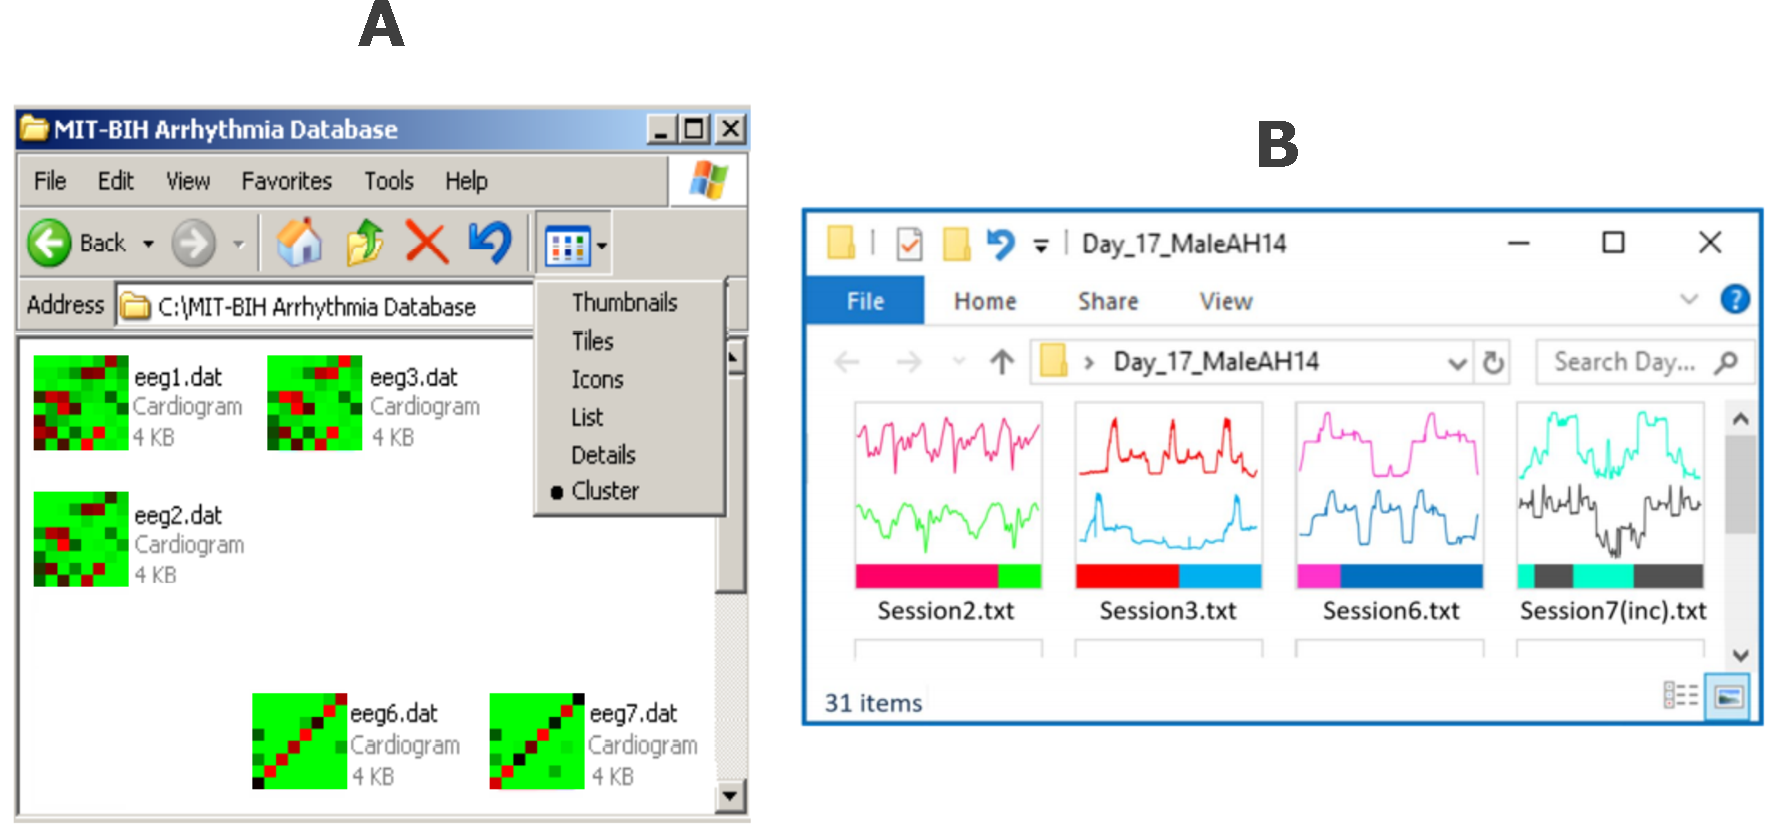
\includegraphics[width=0.8\linewidth]{Figures/keogh_examples.pdf}
    \caption{Strategies for time series summary found on the literature. These images are taken from the works from \cite{snippets, bitmap}}
    \label{fig:keogh_strat}
\end{figure}

Time series \textit{shapelets} are also a method that could provide interesting results. However, the strategy is \textit{supervised}, and the point of the proposed method is to have \textit{no apriori} knowledge about the structure of the data, except the time scale in which the summarization is performed. 
\par
Other interesting strategies provide a transformation of time series into text and could be used for time series summarization, but are not able to suitably summarize a time series from the textual representation \cite{ssts, sax}.



Strategies that are typically used to present information in a compact way are found in several domains. In text analysis, for instance, the relationship between repeating sequences is illustrated with arc diagrams \cite{bitmap, arcplots}. These show where repeating sequences occur in a very concise way. This has a range of applications that include, for example text and DNA sequence analysis.

\begin{figure}[b]
    \centering
    \begin{subfigure}{0.5\linewidth}
    \centering
        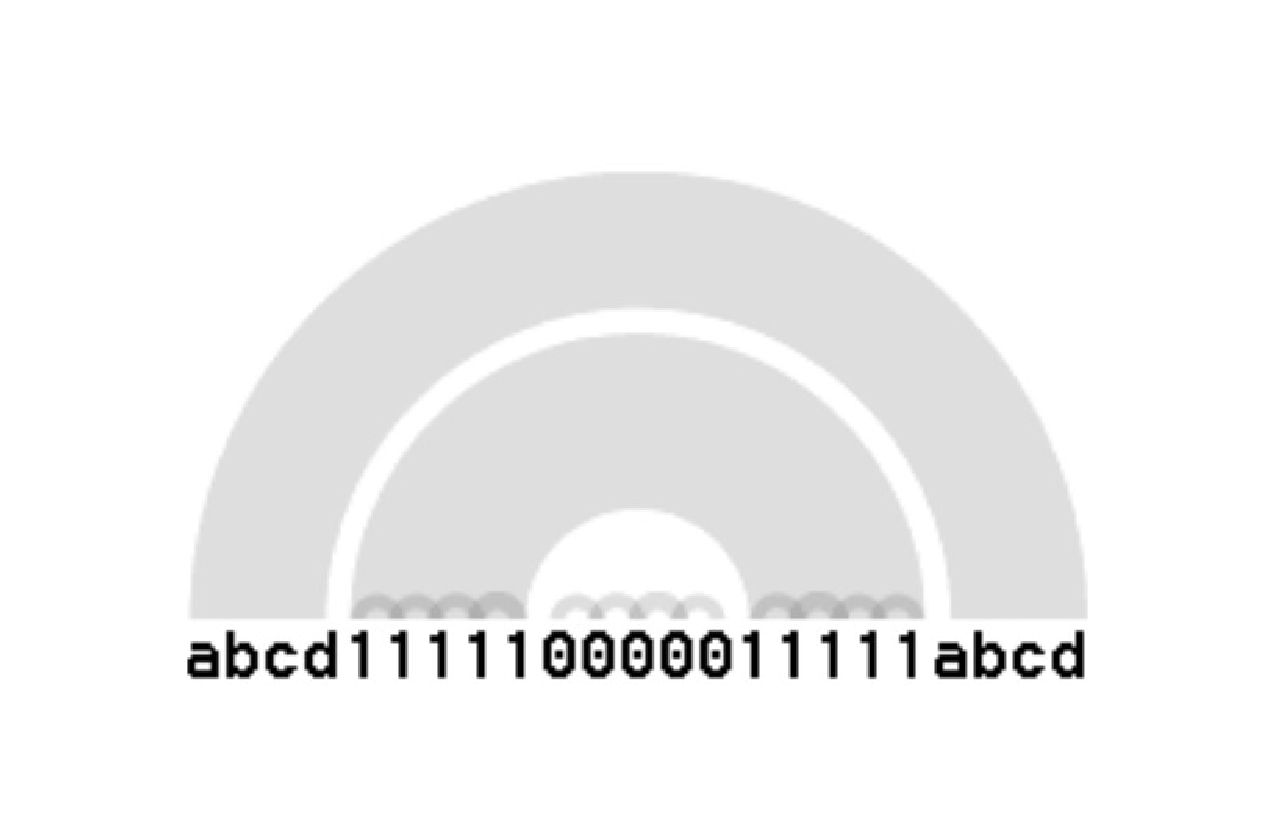
\includegraphics[width=0.9\linewidth]{Figures/arcplots.pdf}
        \caption{}
        \label{fig:genomic}
    \end{subfigure}%
    \begin{subfigure}{0.5\linewidth}
        \centering
        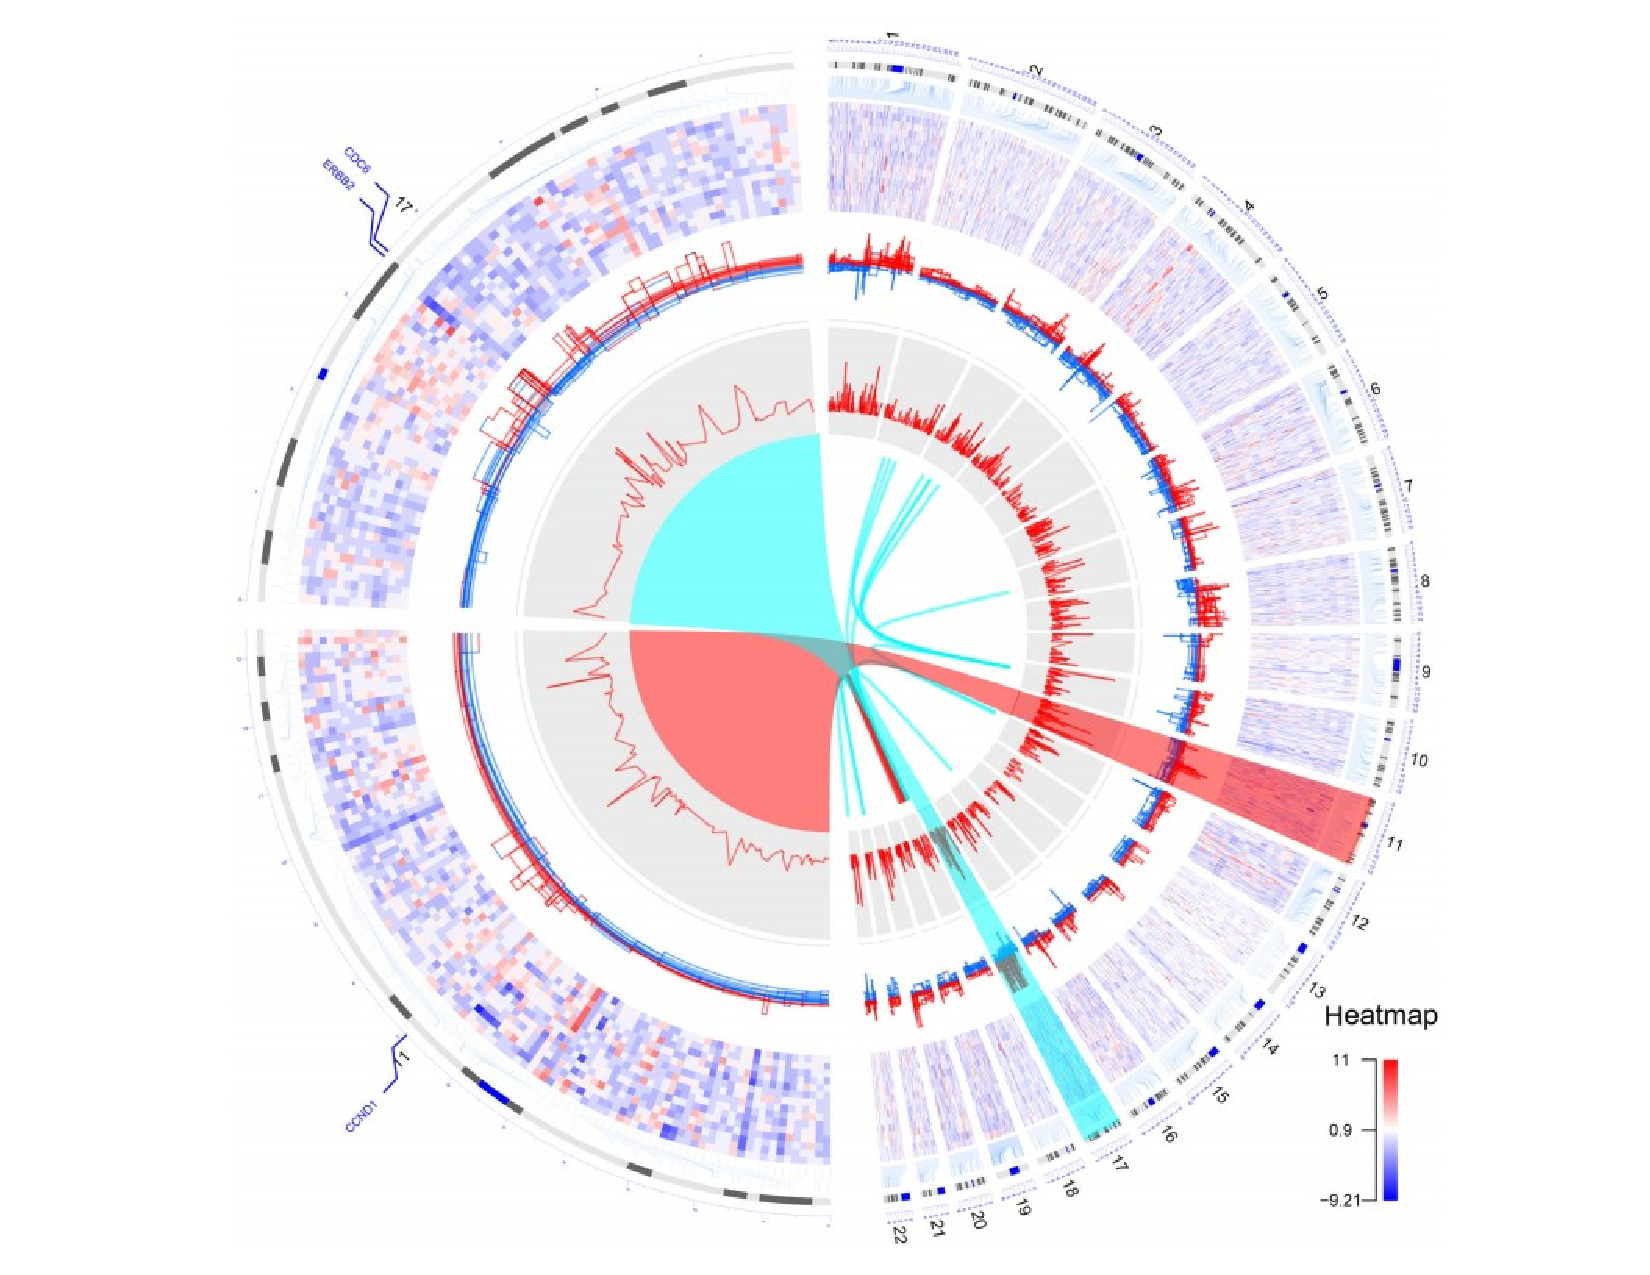
\includegraphics[width=0.9\linewidth]{Figures/genomics.pdf}
        \caption{}
        \label{fig:genomic}
    \end{subfigure}
    \caption{A - Diagram for string association. This image is taken from the works from \cite{arcplots}; B - Circular plot by OmicCircos. Several layers (Circular tracks) identify genome position, expression heatmaps, correlation between expression and CNV, among other features. The image is taken from the works from \textit{Ying Hu, et al.} \cite{genomics}.}
\end{figure}

One domain that has a particular relevance in data visualization is genomics. Graphical genome maps are found to concatenate a significant amount of information in a very compact way. Genome features and sequence characteristics are assessed with this visual strategy. An example can be found on Figure \ref{fig:genomic}. This visualization strategy can provide increasing circular layers of information. Although we are used to look at time series from left to right, a circular representation can have benefits to concatenate the information we want to include.
\par
In the musical domain, strategies have also been developed that summarize audio time series with segmentation techniques. One of the strategies that is common to be used involves detecting novelty instances on a similarity matrix representation of the audio signal, called \textit{Self-Similarity Matrix} (SSM). This data structure provides a significant range of information that can be used to retrieve structural information, such as block and periodic structures \cite{fmp1, fmp2, audiolabs1, audiolabs2}. This method will inspire our visualization strategy, which will be explained further.


\subsection{Classification}

Current available methods for time series classification are categorised as shape-based and structure-based. Existing approaches until the last decade were focused in shape-based similarity methods, while during the mid 2010's, methods that would seek the analysis of higher-level features started to be developed \cite{Keogh2004}.
\par
Shape-based methods focus their attention in performing local comparisons between time series. Examples of well-known methods are the Euclidean distance (ED) or Dynamic Time Warping (DTW) \cite{jlin2013}. Although both work well with short-length time series, the first has the inconvenient of needing time series with the same length, while also being sensitive to time misalignments. The latter is able to counteract this problem by means of determining the best alignment between two time series \cite{Keogh2004, jlin2013}. These distance measures are usually combined with a k-Nearest Neighbour (k-NN) classifier to solve TSC tasks. The limitations of these techniques come with problems that include the presence of noise or long time series with characteristic sub-structures \cite{BOSS}.
\par
In the other end, structure-based methods rely on broader aspects of time series such as the presence of specific morphological structures or patterns, being useful to classify long and noisy time series \cite{BOSS}. Dictionary based methods fit into this category and have recently been used with great success. These techniques rely in a transformation of the time series into a symbolic feature vectors by means of a specific method, such as the \textit{Symbolic Aggregate approXimation} (SAX) \cite{SAX} or the \textit{Symbolic Fourier Approximation} (SFA) \cite{SFA}. The first approach proposed for TSC with symbolic representations was the work of Jessica Lin \textit{et. al} with the \textit{Bag of Patterns} (\textit{BoP})\cite{jlin2013}. Further proposed methods were conceptually inspired on the \textit{BoP}, using the same reasoning. Techniques such as \textit{Bag of SFA Symbols} (BOSS) and Word ExtrAction for time SEries cLassification (WEASEL), from the same authors, use a similar reasoning but employ the SFA instead \cite{BOSS, weasle}.
\par
Using syntactic methods has already been successful for several time series data mining tasks, mostly related with query search and classification. Besides, these methods, being dictionary-based, can be used to show similarity between subsequences by looking into the distribution of word counts. However, current methods rely mostly in incomprehensible sets of characters, such as \textit{aaa}, which are hard to associate with a specific subsequence of the time series, therefore providing limited interpretability. In this work, we propose a method that literally translates the time series into sentences, such as that if a human was to describe a time series with text, it should be possible to separate these time series with the written words. We have seen natural language being used to include the human in the loop for more intuitive and meaningful query searches in time series \cite{hil_naturallanguage}. Such as with SSTS, the purpose is to increase the expressiveness. This kind of descriptive power can be used to provide more intuitive feedback and increase interpretability to understand why a time series is different than others.
\par
There is an existing method that is capable of providing visual interpretability of differences between time series, which is a structure-based method called \textit{shapelets} \cite{shapelets}. Shapelets are representative subsequences of the time series, which characterize a specific class. The advantage of this method is the higher interpretability because relevant shapes from the class can be highlighted \cite{shapelets}. 
\par
All the mentioned methods are a reference in TSC tasks with innovative concepts that merge ideas from the text-mining domain into TSC domain. One of the advantages of structure-based methods that rely in a dictionary-based concept is to use the words extracted as an interpretable model to differentiate time series. The histogram of words generated gives the user an understanding of which patterns better represent the time series and give an intuition over patterns that differ between classes of time series. This provides a feedback and explanation over why a class is different than the other. However, dictionaries can be confusing, and the words generated are not intuitively associated with the patterns these represent in the time series. One method that went beyond the previously mentioned methods in that aspect is the SAX-Vector Space Model (SAX-VSM). This method used a weighted word vector representation of the time series and showed which are the relevant words for the classification process and what patterns these represent in the time series, demonstrating that the classification process can be interpretable by measuring the importance of the patterns found for each class of signals \cite{sax_vsm}. 
\par
The proposed method is built upon the same ideas as the BoP method but uses the \textit{SSTS} Tool to promote the inclusion of the human reasoning in the classification process and provide more interpretable representations, as inspired by the work of SAX-VSM.
\par
The method has been conceptually designed focusing in providing a solution that copes with (1) enabling the human intuition in the classification process, (2) be invariant to size, (3) have awareness of the order at which structures appear on the time series, (4) be domain agnostic, (5) have a flexible pre-processing to increase the representational power and (6) increase the readability. This method brings novelty by using literal natural language sentences to perform classification of time series, which can be customized by an analyst and moves towards a more readable output on distinguishing time series both visually and with keywords.

\subsection{Search by Query}

There is a large literature on time series similarity search, see [26] and the references therein. However, in most cases it is assumed that the query comes from a downstream algorithm, not a human. As such, there has been relatively little attention paid to the ability of humans to formulate meaningful queries. In principle one could do “query-by-sketching” and invite the user to draw the pattern she is interested in finding [15,16]. The recent “Qetch” system is a prominent example of this approach [15]. However, there are two possible limitations to such an approach: First, it is not clear that most people have the ability to sketch their query. For example, many people cannot even draw an accurate circle [25]. Secondly, as Figure 1 hinted at, classic distance measures may be too literal and limited in expressiveness to retrieve the desired pattern. As a simple example, suppose that a user wishes to retrieve all highly symmetric patterns. There is simply no way to do this with Euclidean distance or similar distance measures.
Other researchers have noted these issues and proposed more flexible queries languages for time series. For example, the SDL (shape definition language) of [11]- allows the user to formulate “blurred” queries. However, we believe that most such systems are not accessible for the typical user. For example, in our proposed system, a 3-point-turn can be successfully queried by noting that the surge axis will exhibit three consecutive “bumps” and formulating the query Surge: [peak peak peak]. In contrast, SDL would require: 
(Shape triplespeak (width ht1 ht2 ht3) (in width (in order spike (ht1 ht2 ht3) spike (ht1 ht2 ht3)))). 
Several similar query systems based on regular expressions or SQL-like languages have been proposed, but none seem suitable for general use [17,20].	
There have also been a handful of other attempts at natural language querying for time series [6,7]. None of these works seem to have been adopted by practitioners. We feel that this is because they probably suffer from too broad an ambition, proposing completely domain independent search.  While domain independence is a worthy ambition (and our eventual research goal), it is clearly challenging. Even the word “spike” can have a different meaning for neuroscientists, economists, epidemiologists, and astronomers. In this work we take advantage of the fact that driving is a familiar, even quotidian, activity for most people, and therefore a domain for which most people have strong intuitions for. Moreover, this domain has a near unique property that allows a user to model the behavior they wish to find. We found that, in many cases we could glean intuition as to how a driver’s behavior would reveal itself in telemetry by simply “puppeteering” a smartphone equipped with an app that shows its acceleration and gyroscope readings. For example, by modeling a 3-point turn by sliding the smartphone on a desk, we can see that this behavior best revels itself on the surge axis as three consecutive bumps.


\section{Occupational Health Sensing and Problems} % (fold)
\label{sec:occupai}

% section document_structure (end)
